\documentclass{beamer}[10pt, usepdftitle=false, handout]

\beamertemplatenavigationsymbolsempty

\usepackage[T1]{fontenc}
\usepackage[]{algorithm2e}
\usepackage{multimedia}
\usepackage{gensymb}
\usepackage{textcomp}
\usepackage{background}
%\backgroundsetup{
%    placement=center,
%    scale=1,
%    contents={The author of this course is PAUL BLONDEL},
%    opacity=0.7
%}
%\setbeamertemplate{background}{\BgMaterial}

%\usepackage[font=small,labelfont=bf]{caption} 

\usetheme{Boadilla}

\title{Operating system principles 4}
\author[]{Paul Blondel}
\institute[]{CNAM}
\date[]{September 1st, 2018}

\usepackage[style=british]{csquotes}


\def\signed #1{{\leavevmode\unskip\nobreak\hfil\penalty50\hskip1em
  \hbox{}\nobreak\hfill #1%
  \parfillskip=0pt \finalhyphendemerits=0 \endgraf}}

\newsavebox\mybox
\newenvironment{aquote}[1]
  {\savebox\mybox{#1}\begin{quote}\openautoquote\hspace*{-.7ex}}
  {\unskip\closeautoquote\vspace*{1mm}\signed{\usebox\mybox}\end{quote}}


%\setbeamertemplate{headline}
%{
%  \leavevmode%
%  \hbox{%
%  \begin{beamercolorbox}[wd=1.0\paperwidth,ht=2.25ex,dp=1ex,center]{author in head/foot}%
%    \textcolor{green}{- This course has been made by Paul Blondel -} \usebeamerfont{author in head/foot}\insertsubsection
%  \end{beamercolorbox}}%
%  \vskip0pt%
%}


\setbeamertemplate{footline}
{
  \leavevmode%
  \hbox{%
  \begin{beamercolorbox}[wd=.5\paperwidth,ht=2.25ex,dp=1ex,center]{author in head/foot}%
    \usebeamerfont{author in head/foot}\insertsection
  \end{beamercolorbox}%
  \begin{beamercolorbox}[wd=.5\paperwidth,ht=2.25ex,dp=1ex,center]{title in head/foot}%
    \usebeamerfont{title in head/foot} \inserttitle \hspace*{2em}  \insertframenumber{} / \inserttotalframenumber\hspace*{2ex} 
  \end{beamercolorbox}}%
  \vskip0pt%
}

\AtBeginSection[]
{
   \begin{frame}
    \tableofcontents[ 
    currentsection,
    hideallsubsections] 
   \end{frame}
}

\begin{document}
	{
	\setbeamertemplate{footline}{
  	\leavevmode%
  	\hbox{%
  	\begin{beamercolorbox}[wd=.5\paperwidth,ht=2.25ex,dp=1ex,center]{author in head/foot}%
  	\end{beamercolorbox}%
  	\begin{beamercolorbox}[wd=.5\paperwidth,ht=2.25ex,dp=1ex,center]{title in head/foot}%
  	\end{beamercolorbox}}%
  	\vskip0pt%	
	} 
	\begin{frame}
	\titlepage
	\end{frame}

	\section{Recall}

	\begin{frame}
	
	Recall:
	\vspace*{1em}	
	\begin{itemize}
	\item{The \textit{main memory} is volatile: computer \textbf{turned off = no more data}}	
	\item{\textbf{All programs and data} are stored in the \textit{mass storage memory}}
	\end{itemize}		
	
	\vspace*{1em}	
	
	But how is ensured the conservation / organization of the data in the \textit{mass storage memory}?	
	
	\vspace*{1em}	
	
	\begin{block}{How?}
	This is the goal of the \textbf{File System} (or FS) 	
	\end{block}	
		
	\end{frame}

	\section{Introduction}

	\begin{frame}
	A "file" has \textbf{two representations} in the system:
	\vspace*{1em}
	\begin{itemize}
	\item{The \textbf{"Logical File" representation}: file representation in the \textit{main memory} (what the user can see about the data)}
	\item{The \textbf{"Physical File" representation}: file representation in the \textit{mass storage memory} (data storage)} 
	\end{itemize}
		
	\vspace*{1em}
	
	\begin{block}{What does the FS?}
	The \textbf{FS} handles these two levels of file representation and ensures the matching between the two. 
	\end{block}	
	
	\end{frame}		
			
	\begin{frame}
	
	The "\textit{Logical File}" representation is either:
	\vspace*{1em}	
	\begin{itemize}
	\item{a \textbf{data structure} (as in a programming language) with \textit{creation}, \textit{opening}, \textit{closing} and \textit{destruction} operations:
		\begin{itemize}
		\item{\textbf{creating and opening a logical file: link created} with the \textit{mass storage memory}}
		\item{\textbf{closing and destructing a logical file: cut this link} with the \textit{mass storage memory}}		
		\end{itemize}			
	}
	\vspace*{1em}
	\item{or recordings of data (that can be read from the physical file) with \textbf{three different access modes}:
		\begin{itemize}
		\item{\textbf{sequential mode}, \textbf{indexed mode} and \textbf{direct mode}}	
		\end{itemize}
	}
	\end{itemize}		
			
	\end{frame}
	
	\begin{frame}
	
	The three different modes:
	\vspace*{1em}
	
	\begin{itemize}
	\item{\textbf{Sequential access}: recordings are processed in their order
	\vspace*{0.5em}
	\begin{itemize}
	\item{Here a read operation \textbf{gives the content at the current position}}
	\item{The \textbf{read operation also moves to the next position}\footnotemark[1]}
	\item{A file is accessed either in read only mode or in write mode only}	
	
	\end{itemize}}
	\vspace*{1em}
	\item{\textbf{Indexed access}: recordings can be accessed directly giving a key
	\vspace*{0.5em}
	\begin{itemize}
	\item{The position given is an \textit{access key}}
	\item{For \textbf{each recording: an access key is associated}}
	\item{This access key is \textbf{used to retrieve the right recording}}
	\end{itemize}
	}	
	\vspace*{1em}
	\item{\textbf{Direct access}: Recordings can be accessed directly giving a position
	\vspace*{0.5em}
	\begin{itemize}
	\item{The position is relative to the beginning of the file}
	
	\end{itemize}			
	}	
	
	\end{itemize}		
		
	\footnotetext[1]{This access mode naturally follows HDD physical properties (circular readings and writings on magnetic disks)}	
	
	\end{frame}	
	
	\begin{frame}
	
	The "\textit{Physical file}" representation is:
	\vspace*{1em}
	
	\begin{itemize}
	
	\item{The physical representation as stored in \textit{mass storage memory}}	
	\item{Most \textit{mass storage memories} nowadays are still made of disks (HDD):} 	
	
	\end{itemize}	

	\vspace*{0.5em}	
	
	\begin{center}
		
	\begin{figure}
		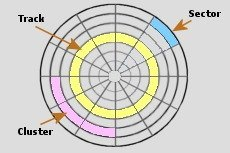
\includegraphics[scale=0.5]{images/sectors.jpg} 
     	%\vspace*{-0.5em}
		%\caption{Floating gate transistor cell}
	\end{figure}
	
	\end{center}	
	
	\pause
	\begin{block}{Optimization}
	Read/write accesses: sectors are \textbf{grouped in clusters} (or blocks)
	\end{block}
	
	\end{frame}	
	
	\begin{frame}
	
	When storing a file into the \textit{mass storage memory}:
	\vspace*{1em}
	\begin{itemize}
	\item{The file is \textbf{stored into \textit{blocks}} (groups of sectors)}
	\item{It becomes a \textit{Physical File}: a set of allocated physical \textit{blocks}}	
	\end{itemize}		
	
	\vspace*{1em}	
	
	Four different approaches to allocate \textit{blocks} in \textit{mass storage memory}:
	\vspace*{0.5em}
	\begin{itemize}
	\item{Contiguous allocation}
	\item{Allocation per area}
	\item{Allocation of linked-blocks}
	\item{Indexed allocation}	
	\end{itemize}
		
	\end{frame}	
	
	\section{Allocation approaches}
	\subsection{Contiguous allocation}	
	
	\begin{frame}
	
	\begin{block}{Contiguous?}
	The file \textbf{must occupy a set of contiguous physical blocks}
	\end{block}
	\vspace*{1em}	
	\begin{itemize}
	\item{Advantages:
		\begin{itemize}
		\item {\textbf{Simple} approach}
		\item {\textbf{Good performances} ("few" physical movements of the reading head)}
		\end{itemize}			
	}	
	\vspace*{1em}
	\item{Drawbacks:
		\begin{itemize}
		\item{Need to know in advance the final file size}
		\item{The memory is \textbf{not optimizely used}\footnotemark[2]}
		\item{The \textbf{fragmentation of the memory is a big problem} here}
		\item{If the \textbf{size of the file increases: big problem}\footnotemark[3]}		
		\end{itemize}
	}			
	\end{itemize}		
	

	\footnotetext[2]{First area, best area and worst area strategies can also be used here}
	\footnotetext[3]{If the size of the file cannot be increased: an error occurs}	
	\end{frame}	

	\subsection{Allocation per area}

	\begin{frame}
		
	\begin{block}{Per area?}
	Here file \textit{blocks} are allocated in two areas: 
	\begin{itemize}
	\item{a primary area (containing the main blocks)}
	\item{a secondary area (useful if the file size increase)}
	\end{itemize}
	\end{block}
	
	\vspace*{1em}	
	
	\begin{itemize}
	
	\item{\textbf{Advantages}:
		\begin{itemize}
			\item{\textbf{More flexibility} to allocate blocks if the file size increases}
		\end{itemize}			
	}\vspace*{0.5em}
	
	
	\item{\textbf{Drawbacks}: 
		\begin{itemize}
			\item{\textbf{More physical movements} of the reading head (slow down a little)}
			\item{We cannot extend too much the secondary area (\textbf{not that flexible}!)}
		\end{itemize}			
	}	
	
	\end{itemize}		
	
	
	\end{frame}
	
	\subsection{Linked-blocks allocation}	
	
	\begin{frame}
	
	\begin{block}{Linked-blocks?}
	File blocks are \textbf{linked together} (each block contains address of next block)\footnotemark[4]	
	\end{block}
	\vspace*{1em}		
		
	\begin{itemize}
	
	\item{\textbf{Advantages}: 
		\begin{itemize}
			\item {\textbf{Extending a file is easy}, we just: add a new block and link it}
			\item {The \textbf{fragmentation of the memory}: is not a problem any longer!}
			\item {\textbf{Don't need to know the final memory size} of the file}		
		\end{itemize}			
	}
	\vspace*{0.5em}
	
	\item{\textbf{Drawbacks}:
		\begin{itemize}
		\item{Can \textbf{only be used in sequential access mode}}
		\item{\textbf{Addresses take place} in the blocks (waste of space!)}
		\end{itemize}
	}	
	
	\end{itemize}			
	
	\footnotetext[5]{A variant to this approach is the FAT (File Allocation Table) approach: here a table keeps the next block positions of each file (the last next block position being identifiable) }
	
		
	\end{frame}	

	\subsection{Indexed allocation}	
	\begin{frame}
	
	\begin{block}{Indexed allocation}
	It \textbf{removes two drawbacks of the linked-blocks allocation approach}!	
	\end{block}
	
	\vspace*{1em}	
	
	All block addresses are stored in one specialized block (named \textit{index}):
	
	\vspace*{1em}
	\begin{center}
	\begin{figure}
		\includegraphics[scale=0.05]{images/indexed.png} 
     	%\vspace*{-0.5em}
		%\caption{Floating gate transistor cell}
	\end{figure}	
	\end{center}
	
	
	\end{frame}
		
	\begin{frame}
	
	If not enough space in one block to store all the addresses, we use \textbf{multilevel indexing}:
	\vspace*{1em}
	\begin{center}
	\begin{figure}
		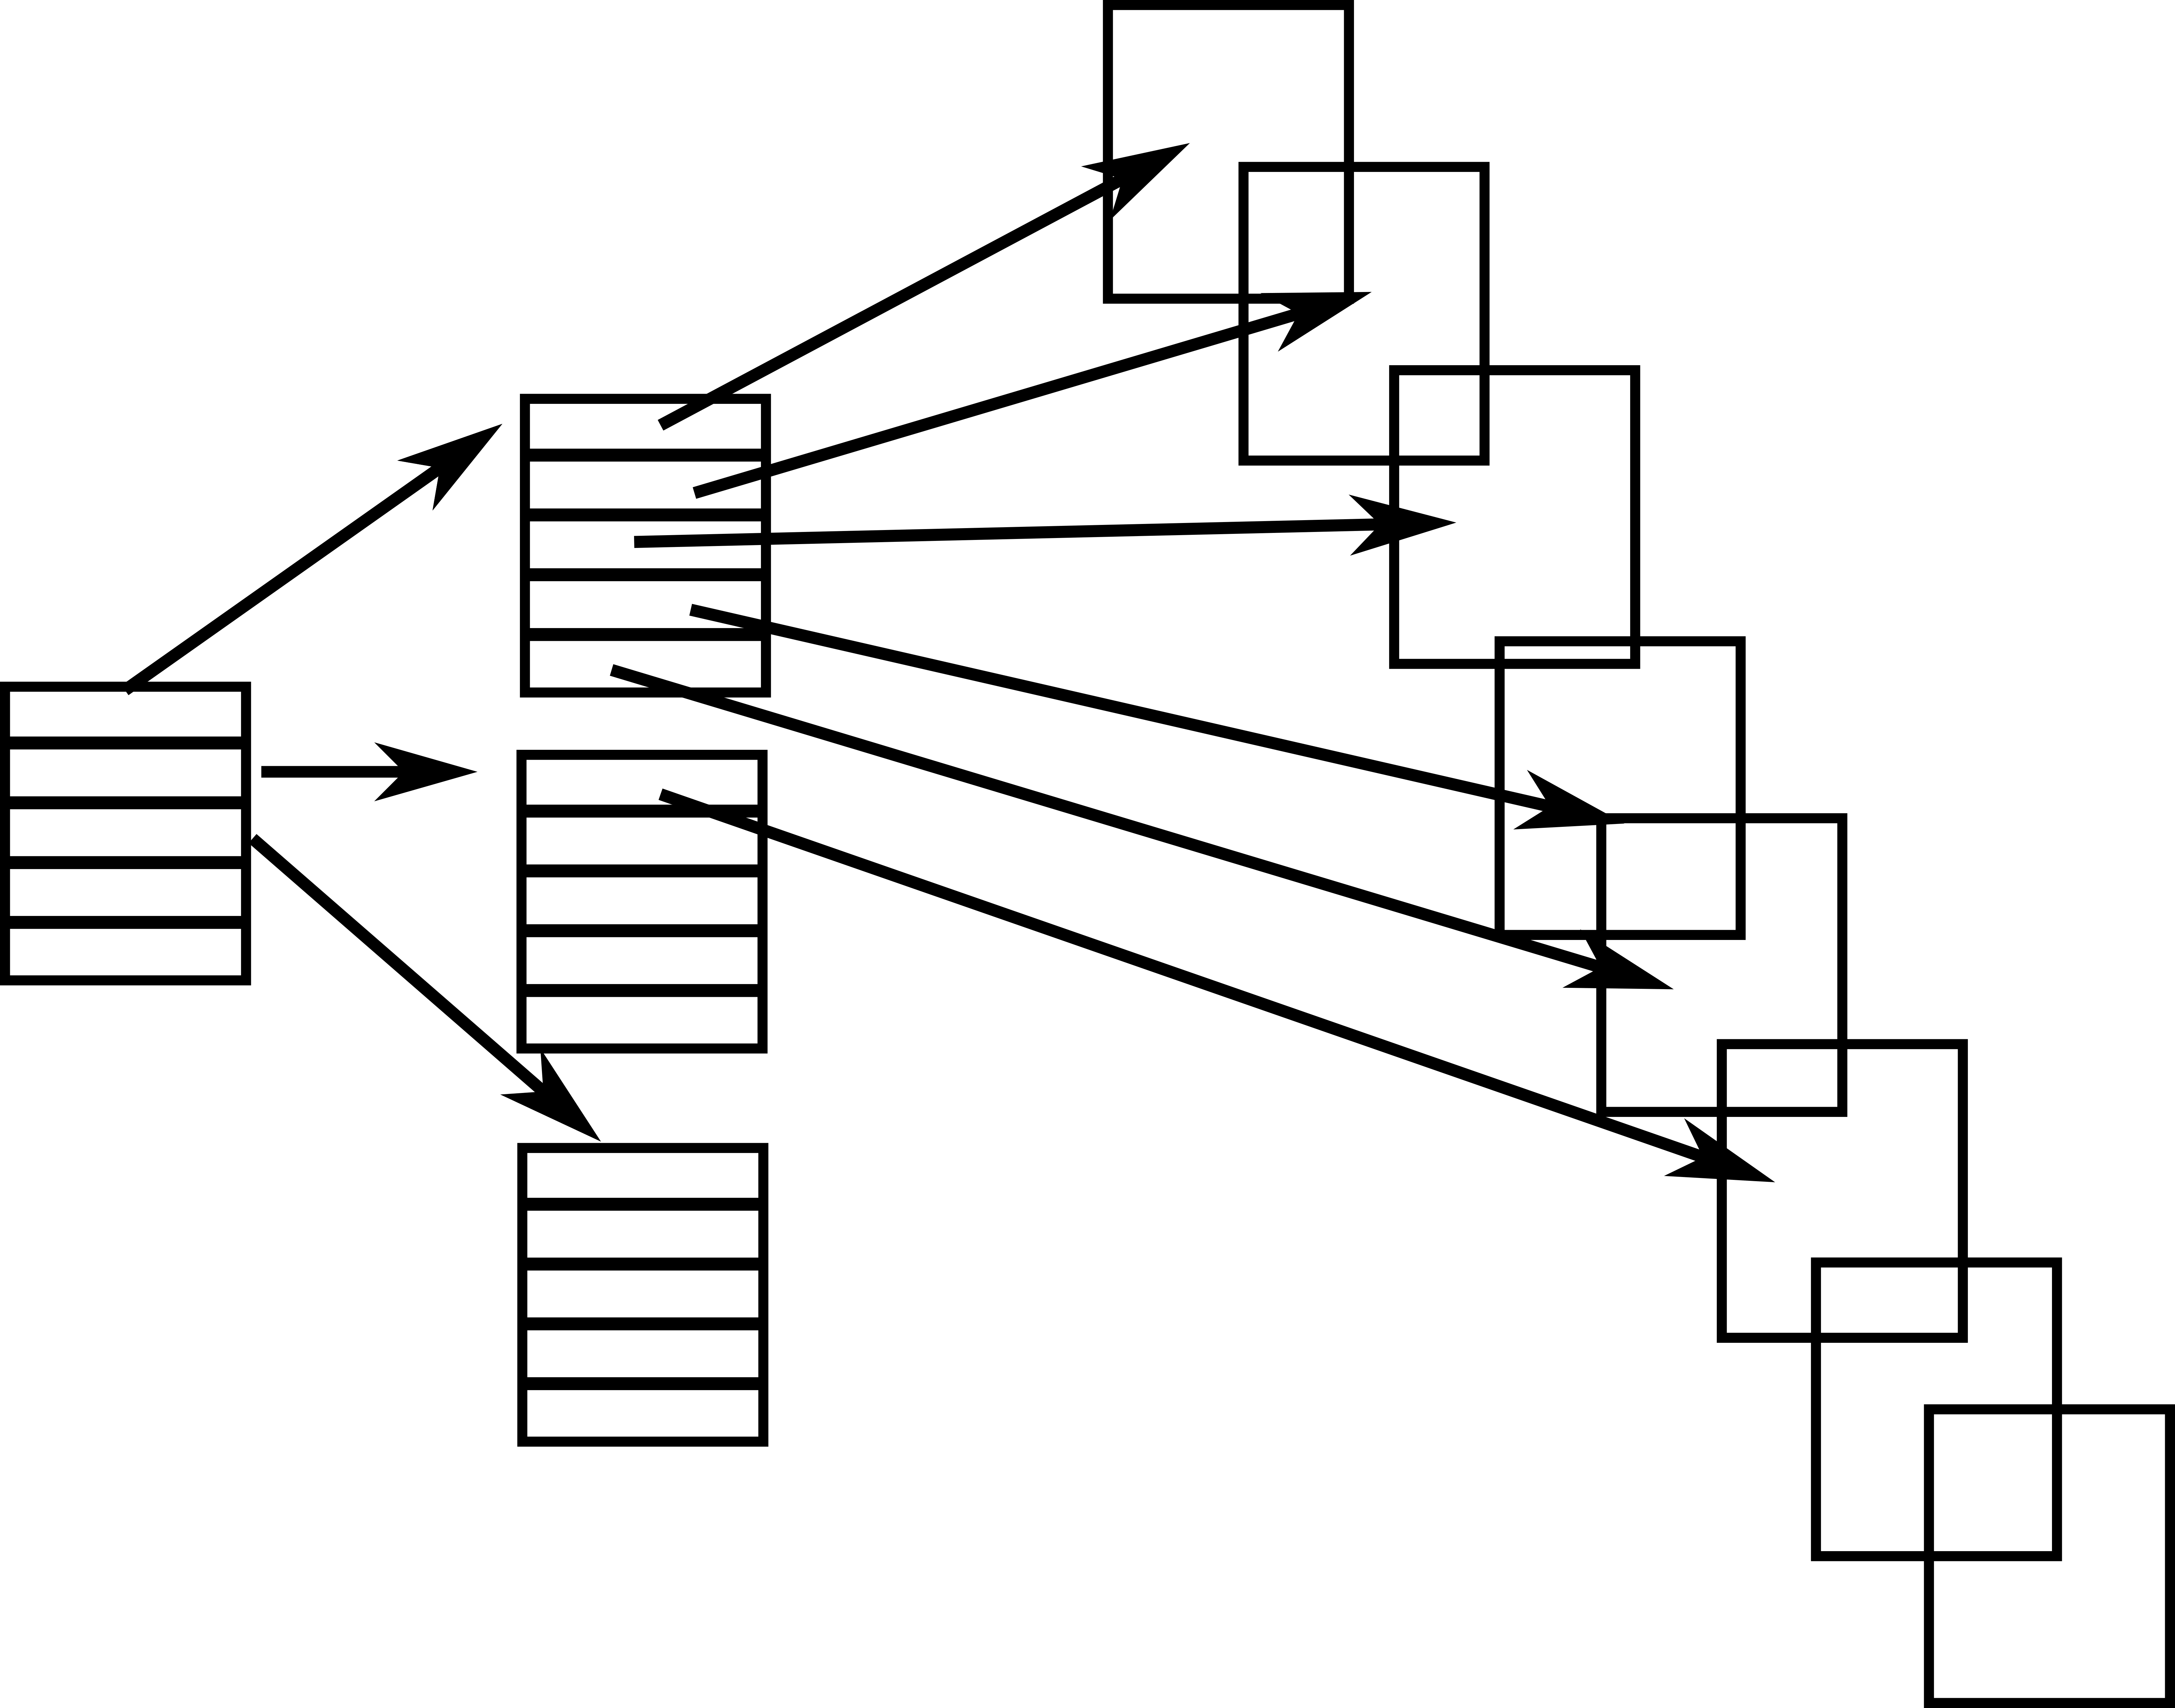
\includegraphics[scale=0.05]{images/indexed2.png} 
     	%\vspace*{-0.5em}
		%\caption{Floating gate transistor cell}
	\end{figure}	
	\end{center}
	
		
	
	\end{frame}		
		
	\begin{frame}
	
	On \textit{UNIX} a modified \textit{indexed allocation} approach is used:
	\vspace*{1em}		
	
	\begin{center}
	\begin{figure}
		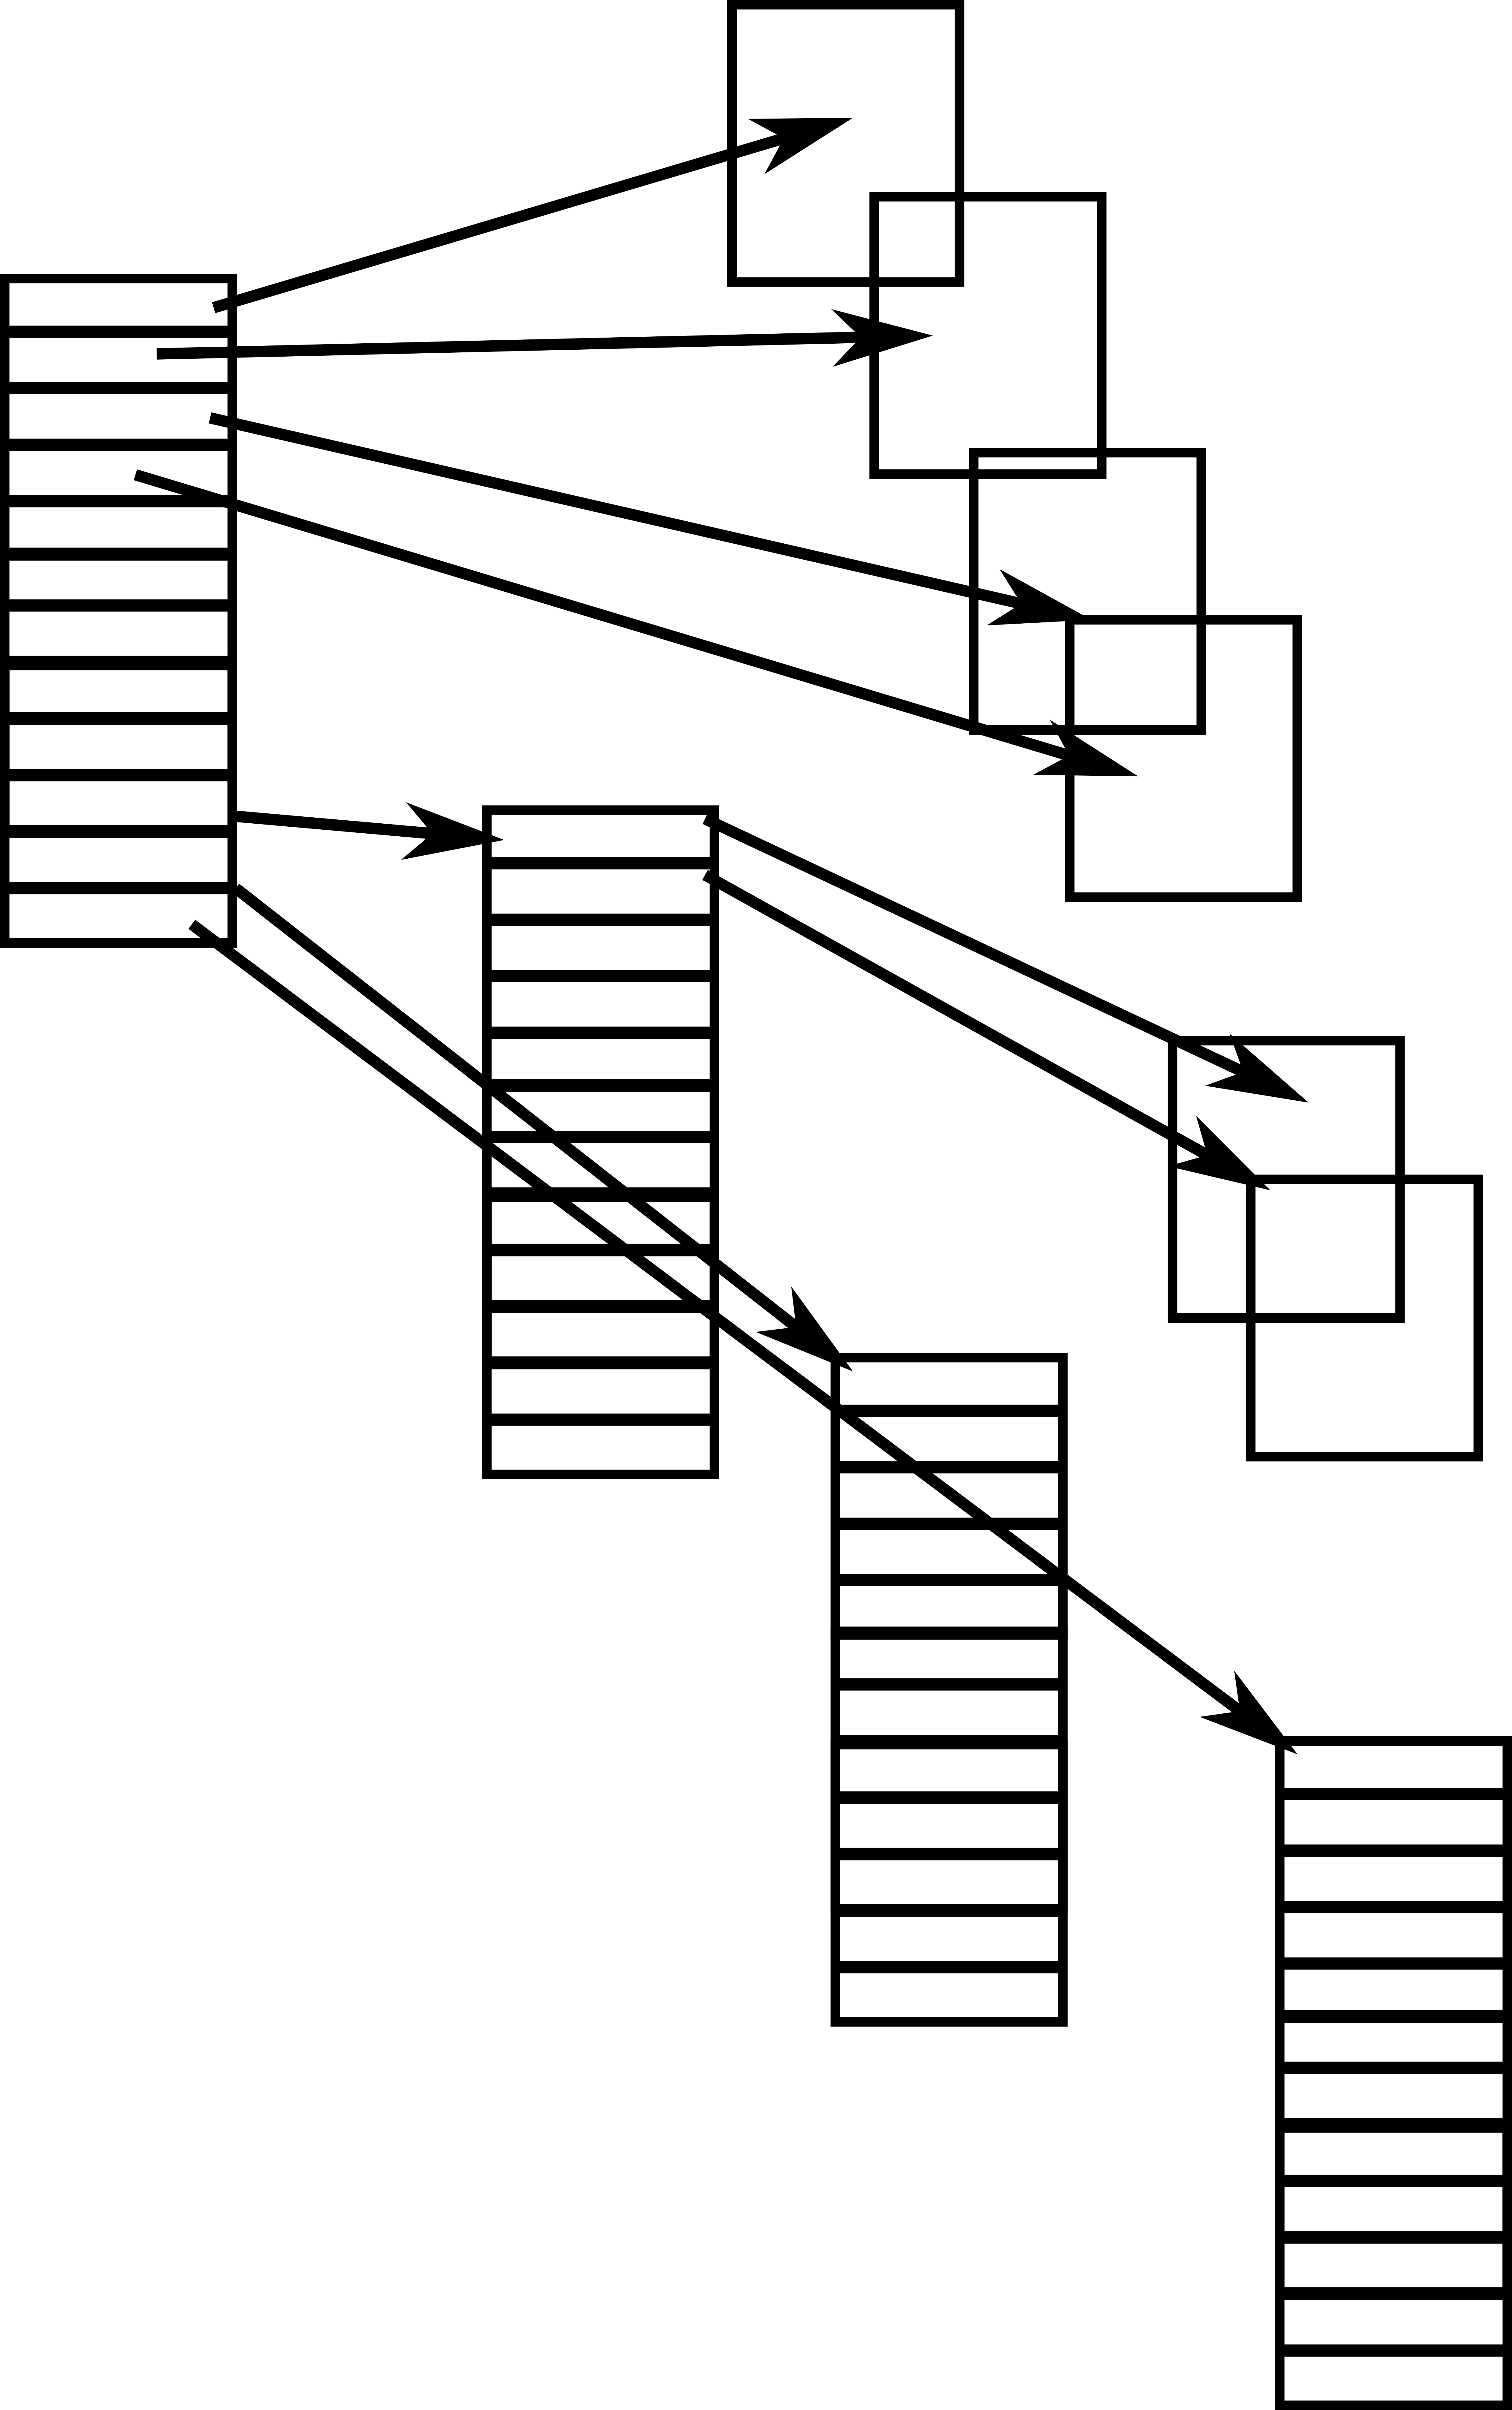
\includegraphics[scale=0.04]{images/indexed3.png} 
     	%\vspace*{-0.5em}
		%\caption{Floating gate transistor cell}
	\end{figure}	
	\end{center}
			
	
	
	\begin{itemize}
	\item{First block is an index with 13 entries}
	\item{10 first entries: addresses to blocks}
	\item{3 last blocks: redirect to other index blocks}	
	\end{itemize}		
		
	
	\end{frame}		
	
	\section{Free space management}
		
	\begin{frame}
	\begin{block}{Free space management?}
	Managing free \textit{blocks} is necessary to find them later and allocate memory
	\end{block}	
	\vspace*{1em}
		
	\begin{itemize}
	\item{When creating a new file: the FS looks for free blocks in a list}
	\item{When a file is destructed: new free blocks are "memorized" in a list}
	\end{itemize}			
	\vspace*{1em}
	There are two ways to identify the list of free blocks\footnotemark[5]:
	\vspace*{0.5em}	
	\begin{itemize}
	\item{using a \textbf{vector of bits}}
	\item{by \textbf{linking the free blocks together}}	
	\end{itemize}		
	
	\footnotetext[5]{With \textit{FAT}: there is already this information in another column of the table of blocks}
	\end{frame}		
		
	\begin{frame}
	
	\begin{itemize}
	\item{\textbf{Vector bit management}: 
	\begin{itemize}
		\item{A bit set to \textbf{0 means: the block is free}}
		\item{A bit set to \textbf{1 means: the block is not free}}
		\item{Example: 1 1 0 0 1 1 0 1 1 0 ........ 1 (1st and 2nd block not free, etc)}
		\item{Vector size = number of blocks}	
	\end{itemize}
	}
	\vspace*{1em}
	
	\item{\textbf{Linked free blocks management}:
		\begin{itemize}
		\item{Finding \textit{N} free blocks = traverse the linked list}
		\item{Traversing the linked list \textbf{step after step: often slow}}
		\item{Variant: in free blocks are stored the number of following free blocks}
		\item{Jumping \textit{M} consecutive free blocks = faster traversal}
		\end{itemize}
	}
	
	\end{itemize}
				
	\end{frame}
	
	\section{Repositories}	
	
	\begin{frame}
	
	\begin{block}{Repository?}
	Repositories contain \textit{FS} information (for some concerned files)
	\end{block}	
	\vspace*{1em}
	The information for each file are:
	\vspace*{0.5em}
	\begin{itemize}
	\item{Name of Logical File}
	\item{Physical address in the mass storage memory (to access the blocks)}
	\item{The file type (.doc, .exe, .o, .gif, etc.)}
	\item{The size of the file (in ko or in block numbers)}
	\item{The name of the file owner}
	\item{Access rights (reading, writing and executing rights)}
	\end{itemize}
	
	\end{frame}	
	
	\begin{frame}
	
	In most \textit{FS}, repositories can have a N-levels structure, here with 2-levels:	
	\vspace*{1em}	
	\begin{center}
	\begin{figure}
		\includegraphics[scale=0.05]{images/repositories_rep.png} 
     	%\vspace*{-0.5em}
		%\caption{Floating gate transistor cell}
	\end{figure}	
	\end{center}
	
	
	\end{frame}	
	
	\section{Partitions}
	
	\begin{frame}
	
	\begin{block}{Partitions?}
	The \textit{FS} may contain several thousands of files, in that case:
	\begin{itemize}
	\item{More convenient to \textbf{split the system in partitions}}
	\item{Each partition \textbf{manages its part of the files}}
	\item{It simplifies the management of the data}
	\end{itemize}
	\end{block}	
	
	\vspace*{0.5em}	
	\begin{center}
	\begin{figure}
		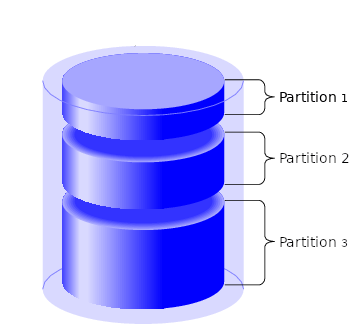
\includegraphics[scale=0.25]{images/hard-disk-partition.png} 
     	%\vspace*{-0.5em}
		%\caption{Floating gate transistor cell}
	\end{figure}	
	\end{center}	
	
	\begin{itemize}
	\item{To access the content of a partition: partition linked to a repository (mounting)}
	\item{When the partition is not needed any longer: link broken with the repository (umounting)}	
	
	\end{itemize}		
		
	
	\end{frame}	
	
	\begin{frame}

	On \textit{UNIX}, a partition is divided as follows:
	\vspace*{1em}	
	\begin{center}
	\begin{figure}
		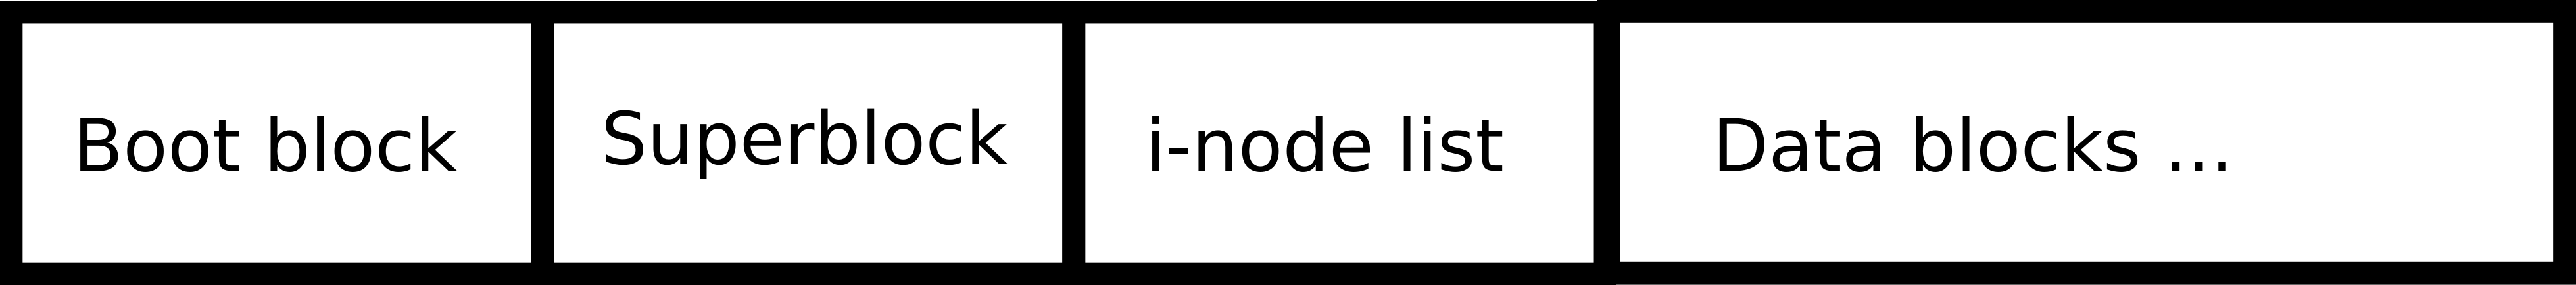
\includegraphics[scale=0.15]{images/unix_part.png} 
     	%\vspace*{-0.5em}
		%\caption{Floating gate transistor cell}
	\end{figure}	
	\end{center}	

	\begin{itemize}
	\item{\textbf{Boot block}: occupy first sector and contains code to initialize the \textit{FS}}
	\item{\textbf{Superblock}: contains information about the \textit{FS} of the partition (\textit{i-node} list, addresses, etc)}
	\item{\textbf{i-node list}: list of \textit{i-nodes} (one \textit{i-node} for each created file in the \textit{FS}}
	\end{itemize}
	
	\vspace*{1em}
	A file is physically represented by a descriptor called "\textit{i-node}"
	
	\vspace*{0.5em}
	An \textit{i-node} contains: the id of the file owner, the file type and the address to the first 13 entries index block.
	\vspace*{1em}
		
	
	\end{frame}		
	
	\section{File system operations}
	\begin{frame}
	Operations on the \textit{FS} can be grouped in two categories:
	\vspace*{1em}
	\begin{itemize}
	\item{operations on files}
	\item{internal operations in files}
	\end{itemize}		
	\vspace*{1em}	
	Operations on files:	
	\vspace*{0.5em}
	\begin{itemize}
	\item{\textbf{creating a file}:
		\begin{itemize}
		\item{\textit{FS} \textbf{checks if a file with the same name does not already exist} in the current repository}
		\item{If not: \textit{FS} \textbf{adds entry to repository and allocate blocks} in mass storage memory}
		\end{itemize}			
	}
	\item{\textbf{opening a file}:
		\begin{itemize}
			\item{The \textit{FS} \textbf{looks for a file with a specific name} in the current repository}
			\item{If user has the rights to open the file (and if it exists): \textbf{a "Logical File" is created (targeting the "Physical File")}}
		\end{itemize}
	}

	\end{itemize}		
	
	
	\end{frame}	
				
	\begin{frame}
		Operations on files:	
		\vspace*{0.5em}
		\begin{itemize}
		\item{\textbf{closing a file}: 
		\begin{itemize}
			\item{The \textit{FS} \textbf{cut the link between the "Logical File"} (file representation on main memory) and the \textbf{"Physical File"} (file representation on mass storage memory)}
		\end{itemize}	
					}
		\item{\textbf{destroying a file}: 
		\begin{itemize}
			\item{The \textit{FS} \textbf{looks for the file with the corresponding name}}
			\item{If it finds is: the \textbf{corresponding entry removed from index and blocks are freed}}		
		\end{itemize}	
					}
		\end{itemize}
		\vspace*{1em}
		Internal operations on files:	
		\vspace*{0.5em}
		\begin{itemize}
		\item{\textbf{read/write operations on a file}: 
		\begin{itemize}
			\item{The \textit{FS} \textbf{keeps track of the next current block position}: to read a new block or to write a new block}
		\end{itemize}	
					}
		\end{itemize}
		
	\end{frame} 
	
	\section{Protections}	
	\begin{frame}
	\begin{block}{Why a protection?}
	The \textit{FS} needs to be protected against two things:
	\begin{itemize}
	\item{\textbf{Inappropriate file accesses} (no right to open/read or execute a file)}
	\item{\textbf{Physical damages}}
	\end{itemize}
	\end{block}
	\vspace*{1em}
	\textbf{Protection against inappropriate file accesses}:
	\vspace*{0.5em} 
		\begin{itemize}
		\item{Files have associated access rights (read, write and execution)}
		\item{Files have an associated access list containing: 
		\begin{itemize}
			\item{explicit user names}
			\item{and/or groups (of user names)}
		\end{itemize}
		
		}		
		
		\end{itemize}
		
	\vspace*{1em}
	Example after a "ls -l" command :
	\vspace*{0.5em}
	
	\begin{tabular}{ccccccc}
	owner & group & all & owner & size & date & filename \\
	rw- & r- - & r- - & name & size1 & date1 &  file1 \\
	rwx & r-x & r-x & name & size2 & date2 & file2
	\end{tabular}
	
	\end{frame}	
	
	\begin{frame}
	\textbf{Protection against physical damages}: 
	\vspace*{0.5em}
	\begin{block}{Useful?}
	YES: power cuts, mechanical damages of the disks, dust, high temperatures, etc ... 
	\end{block}	
	\vspace*{0.5em}
	The \textit{FS} can be protected using two kinds of \textbf{redundancy} techniques:
	\vspace*{1em}	
	\begin{itemize}
	\item{\textbf{Internal redundancy}: two copies of the same data are kept in memory (example: two copies of the FAT) and synchronized at each change}
	\item{\textbf{Periodic saves redundancy}: a copy is kept on another memory device (external hard drive) and it is synchronized at each change (on \textit{UNIX}: the \textit{rsync} command)}	
	\end{itemize}
		
	\end{frame}	
	
			
\end{document}
